% Provenance (never printed): see sources/outline_sources.md (Year 3:
% sequence stratigraphy, accommodation and supply, systems tracts,
% cyclostratigraphy). Brief: sources/book5/BRIEFS.md, ch. 16. Curves from
% figdata/bachelor-3/shelf_model.py and lr04_periodogram.py. Exercise and
% problem values in the Book 5 scratch calculator calc/ch16.py. The Varden
% basin, its shelf and its core are invented.
\chapter{Sequence Stratigraphy}\label{ch:b3:sequence-stratigraphy}

Across a seismic section of a continental margin, reflections lap onto older
ones, then build out toward the basin, then step back toward the land, and
the pattern repeats itself higher up. Each package records a contest between
two rates: the rate at which room for sediment is made, by subsidence and by
the rise of the sea, and the rate at which rivers fill it. Sequence
stratigraphy reads the contest from the geometry of the layers, and
\omterm{def:b3:sequence-stratigraphy:cyclo}{cyclostratigraphy} reads its clock from their thickness.

\begin{recall}
Accommodation, eustasy, relative sea level, subsidence and the sedimentary
basin are in the Year 1 volume, in its chapter on diagenesis and sedimentary
basins. Marine transgression and regression and the first-order sea-level
cycle are in the Year 2 volume, in its chapter on the Phanerozoic Earth; the
Milankovitch parameters and climatic precession in its chapter on orbital
forcing and the ice ages; the age model in its chapter on climate archives
and proxies. \omterm{def:b3:exploration-seismology:terminations}{Onlap}, \omterm{def:b3:exploration-seismology:terminations}{downlap}, \omterm{def:b3:exploration-seismology:terminations}{toplap}, \omterm{def:b3:exploration-seismology:terminations}{erosional truncation} and \omterm{def:b3:exploration-seismology:seismic-stratigraphy}{seismic
stratigraphy} are in Chapter~\ref{ch:b3:exploration-seismology}. Fourier
series and the Fourier transform are in the mathematics books.
\end{recall}

\section{Accommodation, supply and the shoreline}\label{sec:b3:sequence-stratigraphy:shoreline}

At any point of a basin the relative sea level rises at the rate $A = \dot E
+ \sigma$, the eustatic rate plus the subsidence rate (a fall when $A < 0$).
Relative sea level at a place is set by the global sea level and by
everything that moves the land beneath it: \omterm{def:b3:lithosphere-thermal-models:thermal-subsidence}{thermal subsidence}, the load of
the sediment and the flexure it causes, the rebound of the crust after an ice
sheet melts, and the slow push of the mantle beneath the plate. Rising
relative sea level makes accommodation; sediment fills it. Whether the
shoreline moves seaward or landward depends on both, and not on the sea level
alone.
% ledger: miller20:rsl

\begin{definition}[Normal and forced regression]\label{def:b3:sequence-stratigraphy:regression}
A \emph{normal regression}\index{normal regression} is a seaward move of the
shoreline while the relative sea level rises: supply outpaces the
accommodation made at the shoreline. A \emph{forced regression}\index{forced regression}
is a seaward move driven by a fall of relative sea level: the
shoreline is pushed basinward whatever the supply, and the land left behind
is exposed and eroded.
\end{definition}

\begin{definition}[Shoreline trajectory]\label{def:b3:sequence-stratigraphy:trajectory}
The \emph{shoreline trajectory}\index{shoreline trajectory} is the path of
the shoreline through time, drawn in a dip section in the frame of the
sediment, so that it shows both the horizontal move of the shoreline and its
rise or fall relative to the layers below.
\end{definition}

A simple profile makes the contest exact. Behind the shoreline a flat topset
of width $W$ lies at sea level; in front of it a foreset of slope
$\tan\theta$ runs down to the basin floor, a height $D$ below. The sediment
supply $Q$ is a volume per unit time per metre of coastline (an area per unit
time in the section).

\begin{proposition}[Shoreline trajectory]\label{prop:b3:sequence-stratigraphy:trajectory}
If relative sea level rises ($A \ge 0$) and the topset aggrades uniformly,
the shoreline moves at
\[
\frac{\mathrm dx_s}{\mathrm dt} = \frac{Q - AW}{D};
\]
it progrades while $Q > AW$ and retreats when $AW > Q$. If relative sea level
falls ($A < 0$), the topset receives nothing and
\[
\frac{\mathrm dx_s}{\mathrm dt} = \frac{Q}{D} + \frac{|A|}{\tan\theta}.
\]
In both cases the trajectory climbs or descends at the angle whose tangent is
$A/(\mathrm dx_s/\mathrm dt)$.
\end{proposition}

\begin{proof}
In a time $\mathrm dt$ the topset needs $AW\,\mathrm dt$ of sediment to stay
at sea level. What is left, $(Q - AW)\,\mathrm dt$, is spread on the foreset,
a wall of height $D$, which advances by $(Q - AW)\,\mathrm dt/D$; a negative
remainder means the sea floods the topset faster than it fills. When the sea
falls, the topset is above water and receives nothing, and the shoreline
slides down the old foreset by $|A|\,\mathrm dt/\tan\theta$ without any
sediment, while the whole supply builds the foreset forward by $Q\,\mathrm
dt/D$. The shoreline rises by $A\,\mathrm dt$ relative to the layers below
while it moves by $\mathrm dx_s$, which gives the angle.
\end{proof}

A \omterm{def:b3:sequence-stratigraphy:regression}{normal regression} therefore needs a supply larger than the accommodation
made on the topset, and its trajectory climbs; a \omterm{def:b3:sequence-stratigraphy:regression}{forced regression} happens
whatever the supply, and its trajectory descends. The ratio of the two rates,
often written $A/S$, sorts the patterns: progradation when $A/S < 1$ on the
topset, aggradation near 1, retrogradation above. The same sea-level curve
can therefore give a regression on a margin rich in sediment and a
transgression on a starved one.

\section{Stratal geometry: sequences and systems tracts}\label{sec:b3:sequence-stratigraphy:sequences}

The \omterm{def:b3:exploration-seismology:terminations}{reflection terminations} of Chapter~\ref{ch:b3:exploration-seismology}
are the vocabulary of the method: \omterm{def:b3:exploration-seismology:terminations}{onlap} and \omterm{def:b3:exploration-seismology:terminations}{downlap} mark the base of a
package, \omterm{def:b3:exploration-seismology:terminations}{toplap} and \omterm{def:b3:exploration-seismology:terminations}{erosional truncation} its top. Read in a dip section, they
divide a margin into packages bounded by surfaces of non-deposition or
erosion, each recording one cycle of relative sea level.

\begin{definition}[Depositional sequence and sequence boundary]\label{def:b3:sequence-stratigraphy:sequence}
A \emph{depositional sequence}\index{depositional sequence} is a succession
of genetically related strata, without major break inside, bounded at its base
and top by unconformities or by the conformities that continue them into the
basin. Its bounding surface is the \emph{sequence
boundary}\index{sequence boundary}: an unconformity cut by exposure and
erosion on the shelf during a fall of relative sea level, passing basinward
into a correlative conformity.
\end{definition}

\begin{definition}[Systems tract]\label{def:b3:sequence-stratigraphy:tract}
A \emph{systems tract}\index{systems tract} is the set of depositional
systems (river, coast, shelf, slope) that were active together during one
part of a relative sea-level cycle, recognised by its position in the
sequence, its bounding surfaces and its stacking pattern. Four are
distinguished:
\begin{itemize}
\item the \emph{falling-stage systems tract}\index{falling-stage systems tract},
  built by \omterm{def:b3:sequence-stratigraphy:regression}{forced regression} while relative sea level falls:
  downstepping foresets detached from the old shelf;
\item the \emph{lowstand systems tract}\index{lowstand systems tract},
  built by \omterm{def:b3:sequence-stratigraphy:regression}{normal regression} once relative sea level starts to rise again,
  at the lowest shoreline position: a wedge that aggrades and progrades;
\item the \emph{transgressive systems tract}\index{transgressive systems tract},
  built while the shoreline retreats landward: backstepping units
  onlapping the old shelf;
\item the \emph{highstand systems tract}\index{highstand systems tract},
  built by \omterm{def:b3:sequence-stratigraphy:regression}{normal regression} late in the rise, when supply again outpaces
  accommodation: foresets that prograde and \omterm{def:b3:exploration-seismology:terminations}{downlap} onto the deposits below.
\end{itemize}
\end{definition}

\begin{definition}[Transgressive and maximum flooding surfaces]\label{def:b3:sequence-stratigraphy:surfaces}
The \emph{transgressive surface}\index{transgressive surface} is the first
significant \omterm{def:b3:sequence-stratigraphy:parasequence}{flooding surface} above the lowstand deposits: it marks the turn
of the shoreline from regression to transgression. The \emph{maximum flooding
surface}\index{maximum flooding surface} marks the most landward position of
the shoreline, the turn from transgression to highstand regression; the
highstand foresets \omterm{def:b3:exploration-seismology:terminations}{downlap} onto it.
\end{definition}

\begin{definition}[Condensed section and incised valley]\label{def:b3:sequence-stratigraphy:condensed}
A \emph{condensed section}\index{condensed section} is a thin interval
deposited very slowly far from the shoreline while the sea floods the shelf
and the sediment is trapped near the coast: a few centimetres or decimetres
of clay, fossils, glauconite or phosphate that may record a long time. An
\emph{incised valley}\index{incised valley} is a river valley cut into the
exposed shelf while relative sea level falls, and filled during the
following lowstand and transgression.
\end{definition}

\begin{omfigure}
\begin{tikzpicture}[font=\scriptsize, x=0.9cm, y=1.25cm, >=Stealth]
% older highstand deposits below the sequence boundary
\fill[black!10] (0,0) -- (14,0) -- (14,0.4) -- (10,0.6) -- (6,2.8) -- (0,3.0) -- cycle;
\draw[black!35] (1.5,2.0) .. controls (3.2,1.95) and (4.5,1.2) .. (8.5,0.45);
\draw[black!35] (3.5,2.93) .. controls (4.8,2.85) and (6,1.6) .. (10.5,0.42);
% falling-stage systems tract
\fill[red!25] (6.0,2.8) -- (7.4,2.25) -- (8.4,1.85) -- (9.4,1.35) -- (10.4,0.75) -- (10.6,0.58) -- (10,0.6) -- cycle;
\draw[red!60!black] (6.6,2.56) .. controls (7.0,2.4) and (7.5,1.95) .. (8.0,1.70);
\draw[red!60!black] (7.6,2.17) .. controls (8.0,2.0) and (8.5,1.45) .. (9.0,1.15);
\draw[red!60!black] (8.6,1.75) .. controls (9.0,1.55) and (9.5,0.9) .. (10.0,0.6);
% lowstand wedge
\fill[orange!40] (9.2,1.45) -- (10.4,1.5) -- (11.5,1.0) -- (12.6,0.6) -- (13.4,0.44) -- (10.6,0.58) -- (10.4,0.75) -- cycle;
% incised valley and its fill
\fill[orange!30] (2.9,2.9) .. controls (3.3,2.3) and (3.9,2.3) .. (4.3,2.86) -- cycle;
% transgressive systems tract
\fill[green!45!black!35] (11.5,1.0) -- (10.4,1.5) -- (9.2,1.45) -- (8.4,1.85) -- (7.4,2.25) -- (6.0,2.8) -- (1.0,2.97) -- (1.0,3.05) -- (6.0,2.95) -- (7.6,2.5) -- (9.4,1.75) -- (10.8,1.45) -- cycle;
% highstand systems tract
\fill[blue!22] (0,3.62) -- (7.5,3.42) -- (9.8,2.2) -- (11.2,1.22) -- (10.8,1.45) -- (9.4,1.75) -- (7.6,2.5) -- (6.0,2.95) -- (1.0,3.05) -- (0,3.07) -- cycle;
\draw[blue!60!black] (4.0,3.52) .. controls (5.0,3.45) and (5.8,3.1) .. (6.6,2.79);
\draw[blue!60!black] (5.6,3.47) .. controls (6.6,3.4) and (7.4,2.8) .. (8.2,2.26);
\draw[blue!60!black] (6.8,3.44) .. controls (7.8,3.35) and (8.8,2.4) .. (9.7,1.69);
% surfaces
\draw[red!70!black, very thick] (0,3.0) -- (2.9,2.9) .. controls (3.3,2.3) and (3.9,2.3) .. (4.3,2.86) -- (6.0,2.8) -- (7.4,2.25) -- (8.4,1.85) -- (9.2,1.45);
\draw[red!70!black, very thick, densely dashed] (9.2,1.45) -- (9.4,1.35) -- (10.4,0.75) -- (10.6,0.58) -- (14,0.4);
\draw[green!40!black, thick] (11.5,1.0) -- (10.4,1.5) -- (9.2,1.45);
\draw[blue!60!black, thick] (0,3.07) -- (1.0,3.05) -- (6.0,2.95) -- (7.6,2.5) -- (9.4,1.75) -- (10.8,1.45) -- (11.5,1.03) -- (12.6,0.63) -- (13.4,0.47) -- (14,0.43);
% labels
\node[blue!50!black] at (2.6,3.36) {highstand (HST)};
\node[green!35!black, anchor=south] at (4.8,3.92) {transgressive (TST)};
\draw[green!35!black] (4.8,3.92) -- (4.4,3.01);
\node[red!60!black, anchor=west] at (10.1,2.45) {falling stage (FSST)};
\draw[red!60!black] (10.1,2.45) -- (8.8,1.62);
\node[orange!60!black, anchor=west] at (12.2,1.55) {lowstand (LST)};
\draw[orange!60!black] (12.2,1.55) -- (11.2,0.85);
\node[anchor=north, align=center] at (3.6,2.25) {incised\\ valley};
\node[red!70!black, anchor=north] at (1.4,2.95) {SB};
\node[red!70!black, anchor=north] at (12.0,0.38) {correlative conformity};
\node[blue!60!black, anchor=west] at (12.7,1.1) {MFS};
\draw[blue!60!black] (12.7,1.1) -- (12.1,0.82);
\node[green!40!black, anchor=west] at (11.6,2.0) {TS};
\draw[green!40!black] (11.6,2.0) -- (10.9,1.27);
\node[blue!60!black, anchor=south] at (13.4,0.58) {condensed};
\node[anchor=west, black!60] at (0.2,0.35) {older deposits};
\draw[->] (11.2,3.9) -- (12.6,3.9) node[right] {basinward};
\end{tikzpicture}

\par\smallskip{\small Anatomy of a \omterm{def:b3:sequence-stratigraphy:sequence}{depositional sequence} in a dip section
(schematic, vertical scale much exaggerated). The \omterm{def:b3:sequence-stratigraphy:sequence}{sequence boundary} (SB, red)
is an unconformity on the shelf, with an \omterm{def:b3:sequence-stratigraphy:condensed}{incised valley}, and a correlative
conformity in the basin (dashed); here it is drawn above the falling-stage
deposits. The \omterm{def:b3:sequence-stratigraphy:surfaces}{transgressive surface} (TS) caps the lowstand wedge; the \omterm{def:b3:sequence-stratigraphy:surfaces}{maximum
flooding surface} (MFS) caps the thin transgressive tract and passes basinward
into a \omterm{def:b3:sequence-stratigraphy:condensed}{condensed section}; the highstand foresets \omterm{def:b3:exploration-seismology:terminations}{downlap} onto it.}\label{fig:b3:sequence-stratigraphy:anatomy}
\end{omfigure}

Where exactly the \omterm{def:b3:sequence-stratigraphy:sequence}{sequence boundary} runs in the basin is a convention, and
authors differ: some draw it at the base of the falling-stage deposits, where
the fall begins, others at their top, where it ends, as in the figure above.
On the shelf there is no ambiguity: the boundary is the surface of exposure
and erosion, and the deposits above it are younger than the fall.

Read from the bottom up at one place on the outer shelf, a sequence records
the cycle: highstand foresets, a surface of exposure, perhaps a valley fill,
the \omterm{def:b3:sequence-stratigraphy:surfaces}{transgressive surface}, backstepping beds, a condensed interval at the
\omterm{def:b3:sequence-stratigraphy:surfaces}{maximum flooding surface}, then highstand foresets again. The hierarchy of
cycles is set by their causes: the opening and closing of oceans for the
first-order cycle, changes in ice volume and in the speed of sea-floor
spreading for the shorter ones, and local tectonics and supply for all of
them.

\section{Parasequences and stacking patterns}\label{sec:b3:sequence-stratigraphy:parasequences}

Inside a \omterm{def:b3:sequence-stratigraphy:tract}{systems tract} the smallest packages a geologist maps on a cliff or a
well log are shallowing-upward units a few metres to a few tens of metres
thick, capped by a surface where deeper water suddenly returns.

\begin{definition}[Parasequence and flooding surface]\label{def:b3:sequence-stratigraphy:parasequence}
A \emph{parasequence}\index{parasequence} is a relatively conformable
succession of genetically related beds bounded by flooding surfaces, in which
the water shallows upward: on a wave-dominated coast, offshore mud passes up
into lower and upper shoreface sand and beach. A \emph{flooding
surface}\index{flooding surface} is a surface across which deeper-water
facies abruptly overlie shallower ones, with evidence of a sudden deepening.
\end{definition}

A single \omterm{def:b3:sequence-stratigraphy:parasequence}{parasequence} coarsens upward, and its gamma-ray log, low in sand
and high in clay, makes a funnel shape that narrows upward. How the
\omterm{def:b3:sequence-stratigraphy:parasequence}{parasequences} of a tract stack upon one another tells the trend of the
shoreline: each one built farther seaward than the last (progradational),
above the last (aggradational), or landward of it (retrogradational). A log
through the stack shows the trend directly: each \omterm{def:b3:sequence-stratigraphy:parasequence}{parasequence} ending in
coarser, shallower facies than the one below, the same, or finer and deeper.
Highstand and lowstand tracts stack progradationally or aggradationally,
transgressive tracts retrogradationally. The next chapter reads such logs
facies by facies.

\begin{omfigure}
\begin{tikzpicture}[font=\scriptsize, x=1cm, y=1cm]
% three logs: each parasequence a coarsening-upward wedge (grain size to the right)
% progradational
\begin{scope}[xshift=0cm]
\fill[yellow!45!brown!35] (0,0) -- (0.5,0) -- (1.4,1.1) -- (0,1.1) -- cycle;
\fill[yellow!45!brown!35] (0,1.1) -- (0.5,1.1) -- (1.8,2.2) -- (0,2.2) -- cycle;
\fill[yellow!45!brown!35] (0,2.2) -- (0.5,2.2) -- (2.2,3.3) -- (0,3.3) -- cycle;
\draw (0,0) -- (0.5,0) -- (1.4,1.1) -- (0.5,1.1) -- (1.8,2.2) -- (0.5,2.2) -- (2.2,3.3) -- (0,3.3) -- cycle;
\node[anchor=north, align=center] at (1.1,-0.1) {progradational\\ (shoreline moves seaward)};
\end{scope}
% aggradational
\begin{scope}[xshift=4.2cm]
\fill[yellow!45!brown!35] (0,0) -- (0.5,0) -- (1.8,1.1) -- (0,1.1) -- cycle;
\fill[yellow!45!brown!35] (0,1.1) -- (0.5,1.1) -- (1.8,2.2) -- (0,2.2) -- cycle;
\fill[yellow!45!brown!35] (0,2.2) -- (0.5,2.2) -- (1.8,3.3) -- (0,3.3) -- cycle;
\draw (0,0) -- (0.5,0) -- (1.8,1.1) -- (0.5,1.1) -- (1.8,2.2) -- (0.5,2.2) -- (1.8,3.3) -- (0,3.3) -- cycle;
\node[anchor=north, align=center] at (1.1,-0.1) {aggradational\\ (shoreline stays)};
\end{scope}
% retrogradational
\begin{scope}[xshift=8.4cm]
\fill[yellow!45!brown!35] (0,0) -- (0.5,0) -- (2.2,1.1) -- (0,1.1) -- cycle;
\fill[yellow!45!brown!35] (0,1.1) -- (0.5,1.1) -- (1.8,2.2) -- (0,2.2) -- cycle;
\fill[yellow!45!brown!35] (0,2.2) -- (0.5,2.2) -- (1.4,3.3) -- (0,3.3) -- cycle;
\draw (0,0) -- (0.5,0) -- (2.2,1.1) -- (0.5,1.1) -- (1.8,2.2) -- (0.5,2.2) -- (1.4,3.3) -- (0,3.3) -- cycle;
\node[anchor=north, align=center] at (1.1,-0.1) {retrogradational\\ (shoreline moves landward)};
\end{scope}
% flooding surfaces
\foreach \s in {0,4.2,8.4} {
  \draw[omDef, thick] (\s-0.15,1.1) -- (\s+2.5,1.1);
  \draw[omDef, thick] (\s-0.15,2.2) -- (\s+2.5,2.2);
  \node[omDef, anchor=west] at (\s+2.5,1.1) {FS};
  \node[omDef, anchor=west] at (\s+2.5,2.2) {FS};
}
% grain-size axis
\draw[->] (0,3.6) -- (2.3,3.6) node[right] {coarser};
\node[anchor=east] at (0,3.6) {mud};
\end{tikzpicture}

\par\smallskip{\small Three \omterm{def:b3:sequence-stratigraphy:parasequence}{parasequences} stacked three ways, drawn as
grain-size logs (width to the right means coarser). Each \omterm{def:b3:sequence-stratigraphy:parasequence}{parasequence}
coarsens upward from offshore mud to shoreface sand and ends at a \omterm{def:b3:sequence-stratigraphy:parasequence}{flooding
surface} (FS); the top of each is coarser than the one below when the stack
progrades, the same when it aggrades, finer when it
retrogrades.}\label{fig:b3:sequence-stratigraphy:stacking}
\end{omfigure}

\begin{inthefield}[Parasequences in a desert cliff]
\begin{minipage}[t]{0.52\linewidth}\vspace{0pt}
The Book Cliffs of eastern Utah expose Upper Cretaceous shoreline deposits
for tens of kilometres. In the Kenilworth Member, followed along the cliffs
from Price to Hatch Mesa, geologists mapped coastal-plain, shoreface,
inner-shelf and incised-valley deposits, and nine coarsening-upward,
wave- to storm-dominated \omterm{def:b3:sequence-stratigraphy:parasequence}{parasequences} 7 to \qty{32}{m} thick. Basinward
each splits into up to four smaller coarsening-upward bedsets, 2 to
\qty{18}{m} thick; some shoreface sands rest on a sharp base, which the
study reads as deposits of a lowstand.
\end{minipage}\hfill
\begin{minipage}[t]{0.44\linewidth}\vspace{0pt}
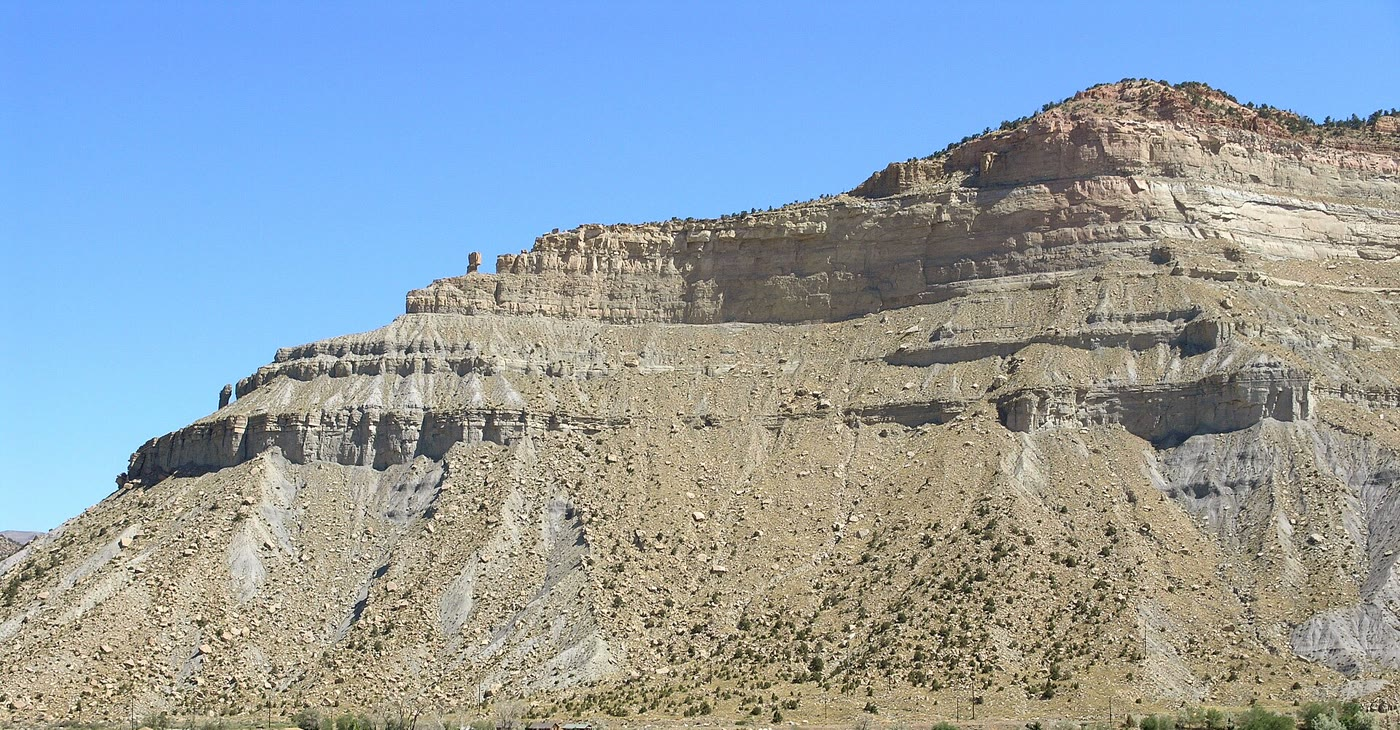
\includegraphics[width=\linewidth]{images/book5/b3-book-cliffs-helper.jpg}

{\scriptsize The Book Cliffs above Helper, Utah: pale sandstone ledges stand
out above grey mudrock slopes. Photo David Mackie, public domain.}
\end{minipage}
\end{inthefield}
% ledger: pattison95:kenilworth, photo:b3-book-cliffs

\section{A forward model of a shelf}\label{sec:b3:sequence-stratigraphy:model}

The rules of the previous sections can be run as a model. The Varden basin
is an invented shelf: a ramp sloping basinward at \qty{1.5}{m/km}, subsiding
at $\sigma = 0.02 + x/1200$ \unit{m/kyr} at a distance $x$ (km) from the
hinge, under a sea level $E = -30\cos(2\pi t/400)$ (m, $t$ in kyr), fed by a
river supplying $Q = \qty{6000}{m^3/kyr}$ per metre of coast. At every step
of half a thousand years the basin subsides; the sediment then fills a flat
topset up to sea level, wherever the old surface is under water, and a
foreset of slope 0.012 in front of it, the shoreline being placed so that the
volume added equals the supply; exposed land receives nothing and, for
simplicity, is not eroded. The model starts at a lowstand, after a first
wedge built at constant sea level.

\begin{omfigure}
\begin{tikzpicture}
\begin{groupplot}[group style={group size=1 by 2, vertical sep=0.35cm, x descriptions at=edge bottom},
  omrecord, width=0.86\linewidth, xmin=0, xmax=600,
  xtick={0,100,200,300,400,500,600},
  tick label style={font=\scriptsize}, label style={font=\small}]
\nextgroupplot[height=0.2\linewidth, ylabel={$E$ (m)}, ymin=-35, ymax=35,
  ytick={-30,0,30}]
\addplot[omDef, thick, domain=0:600, samples=121] {-30*cos(deg(2*pi*x/400))};
\nextgroupplot[height=0.3\linewidth, xlabel={time (kyr)}, ylabel={shoreline $x_s$ (km)},
  ymin=0, ymax=60, ytick={0,20,40,60},
  scatter/classes={1={mark=*, red!70!black}, 2={mark=*, orange!80!black},
    3={mark=*, green!50!black}, 4={mark=*, blue!70!black}}]
% computed in figdata/bachelor-3/shelf_model.py
\addplot[scatter, only marks, mark size=0.9pt, scatter src=explicit symbolic]
  table[x=t, y=xs, meta=tract] {figdata/out/bachelor-3-shelf_model-shore.dat};
\node[font=\scriptsize, orange!60!black] at (axis cs:12,56) {LST};
\node[font=\scriptsize, green!40!black] at (axis cs:70,40) {TST};
\node[font=\scriptsize, blue!60!black] at (axis cs:160,6) {HST};
\node[font=\scriptsize, red!60!black] at (axis cs:300,22) {FSST};
\node[font=\scriptsize, orange!60!black] at (axis cs:415,57) {LST};
\node[font=\scriptsize, green!40!black] at (axis cs:520,45) {TST};
\node[font=\scriptsize, blue!60!black] at (axis cs:580,12) {HST};
\end{groupplot}
\end{tikzpicture}

\par\smallskip{\small Above, the eustatic sea level of the Varden model;
below, the position of the shoreline, coloured by \omterm{def:b3:sequence-stratigraphy:tract}{systems tract} (lowstand
orange, transgressive green, highstand blue, falling stage red), classified
from the model's output alone: falling stage while relative sea level falls
at the shoreline, transgressive while the shoreline retreats, lowstand or
highstand while it advances under a rising sea, after a fall or after a
transgression.}\label{fig:b3:sequence-stratigraphy:series}
\end{omfigure}

The figure above follows the shoreline through time, and the one below
shows the deposits it left. The tracts appear with no rule written into the
model beyond filling and subsidence. The lowstand wedge at the start sits far
out; the rising sea drives the shoreline \qty{38}{km} landward in the first
transgression, and the highstand foresets build out again as the rise slows.
Then the fall begins: the shoreline is pushed basinward by \qty{33}{km} in
\qty{187}{kyr}, leaving thin downstepping foresets and an exposed shelf
behind, the falling-stage tract. A new lowstand wedge, a second transgression
and a new highstand follow. The speed of the \omterm{def:b3:sequence-stratigraphy:regression}{forced regression} in the model
matches the formula of the proposition to within a few per cent; under a
rising sea the model's topset does not aggrade uniformly, since subsidence
grows basinward, and the formula is only a guide.

\begin{omfigure}
\begin{tikzpicture}
\begin{axis}[omsection, width=0.95\linewidth, height=0.42\linewidth,
  xmin=0, xmax=70, ymin=-150, ymax=40, clip=true,
  xlabel={distance basinward (km)}, ylabel={elevation now (m)},
  xtick={0,10,20,30,40,50,60,70}, ytick={-150,-100,-50,0},
  tick label style={font=\scriptsize}, label style={font=\small}]
% computed in figdata/bachelor-3/shelf_model.py
\addplot[fill=black!10, draw=none] table[x=x, y=z0] {figdata/out/bachelor-3-shelf_model-surfaces.dat} -- (axis cs:120,-300) -- (axis cs:0,-300) -- cycle;
\addplot[fill=orange!45, draw=none] table[x=x, y=z] {figdata/out/bachelor-3-shelf_model-poly1.dat};
\addplot[fill=green!45!black!35, draw=none] table[x=x, y=z] {figdata/out/bachelor-3-shelf_model-poly2.dat};
\addplot[fill=blue!25, draw=none] table[x=x, y=z] {figdata/out/bachelor-3-shelf_model-poly3.dat};
\addplot[fill=red!30, draw=none] table[x=x, y=z] {figdata/out/bachelor-3-shelf_model-poly4.dat};
\addplot[fill=orange!45, draw=none] table[x=x, y=z] {figdata/out/bachelor-3-shelf_model-poly5.dat};
\addplot[fill=green!45!black!35, draw=none] table[x=x, y=z] {figdata/out/bachelor-3-shelf_model-poly6.dat};
\addplot[fill=blue!25, draw=none] table[x=x, y=z] {figdata/out/bachelor-3-shelf_model-poly7.dat};
\addplot[black!45, very thin] table[x=x, y=z40] {figdata/out/bachelor-3-shelf_model-surfaces.dat};
\addplot[black!45, very thin] table[x=x, y=z80] {figdata/out/bachelor-3-shelf_model-surfaces.dat};
\addplot[black!45, very thin] table[x=x, y=z120] {figdata/out/bachelor-3-shelf_model-surfaces.dat};
\addplot[black!45, very thin] table[x=x, y=z160] {figdata/out/bachelor-3-shelf_model-surfaces.dat};
\addplot[black!45, very thin] table[x=x, y=z240] {figdata/out/bachelor-3-shelf_model-surfaces.dat};
\addplot[black!45, very thin] table[x=x, y=z280] {figdata/out/bachelor-3-shelf_model-surfaces.dat};
\addplot[black!45, very thin] table[x=x, y=z320] {figdata/out/bachelor-3-shelf_model-surfaces.dat};
\addplot[black!45, very thin] table[x=x, y=z360] {figdata/out/bachelor-3-shelf_model-surfaces.dat};
\addplot[black!45, very thin] table[x=x, y=z440] {figdata/out/bachelor-3-shelf_model-surfaces.dat};
\addplot[black!45, very thin] table[x=x, y=z480] {figdata/out/bachelor-3-shelf_model-surfaces.dat};
\addplot[black!45, very thin] table[x=x, y=z520] {figdata/out/bachelor-3-shelf_model-surfaces.dat};
\addplot[black!45, very thin] table[x=x, y=z560] {figdata/out/bachelor-3-shelf_model-surfaces.dat};
\addplot[black, thin] table[x=x, y=z600] {figdata/out/bachelor-3-shelf_model-surfaces.dat};
\addplot[black, only marks, mark=*, mark size=0.5pt] table[x=xs, y=zfinal] {figdata/out/bachelor-3-shelf_model-shore.dat};
\node[font=\scriptsize, blue!50!black] at (axis cs:6,4) {HST};
\node[font=\scriptsize, green!30!black] at (axis cs:12,-22) {TST};
\node[font=\scriptsize, red!60!black] at (axis cs:35,-25) {FSST};
\node[font=\scriptsize, orange!60!black] at (axis cs:57.5,-60) {LST};
\node[font=\scriptsize, green!30!black] at (axis cs:36,2) {TST};
\node[font=\scriptsize, blue!50!black] at (axis cs:8,26) {HST};
\end{axis}
\end{tikzpicture}

\par\smallskip{\small The Varden shelf after \qty{600}{kyr}, in its present
position (vertical scale exaggerated about 170 times). Colours are the
\omterm{def:b3:sequence-stratigraphy:tract}{systems tracts}: lowstand orange, transgressive green, highstand blue,
falling stage red; grey is the older ramp and the first wedge. Thin lines are
the sea floor every \qty{40}{kyr}; black dots trace the shoreline every
\qty{2}{kyr}. Computed by the forward model of the
text.}\label{fig:b3:sequence-stratigraphy:section}
\end{omfigure}


The relative sea level begins to fall at the shoreline a few thousand years
after the eustatic highstand, because the subsidence must first be overtaken,
and it ends a few thousand years before the eustatic lowstand. The fall at
the shoreline thus lasts less than half the eustatic cycle, and the more so
the faster the basin subsides.

Models of this kind are the honest test of an interpretation, and also show
its limits. The same section can be built by different histories: a faster
fall with less supply, or a slower one with more, or a change of subsidence
rather than of sea level, since the geometry only records the relative sea
level and the supply. Global charts of sea-level cycles built from margins in
the 1970s and 1980s fixed the timing of many falls that drilling has since
largely confirmed for parts of the Late Cretaceous to Miocene, but their
amplitudes, such as a fall of \qty{160}{m} in the middle Oligocene, are too
high by a factor of 2 to 3. Eustatic amplitudes are now taken from
oxygen isotopes and from backstripped wells, and a margin's sequences are
read first as a local record.
% ledger: miller20:epr, miller20:rsl

\section{Cyclostratigraphy}\label{sec:b3:sequence-stratigraphy:cyclo}

Many successions repeat themselves at regular thickness intervals: couplets
of marl and limestone, bundles of five couplets, larger sets of bundles. If
the repetition is paced by the Milankovitch parameters, the thickness of the
cycles turns into time.

\begin{definition}[Cyclostratigraphy and astronomical tuning]\label{def:b3:sequence-stratigraphy:cyclo}
\emph{Cyclostratigraphy}\index{cyclostratigraphy} identifies and measures
regular cycles in sedimentary successions and interprets them as records of
periodic forcing, mainly the variations of the Earth's orbit and axis.
\emph{Astronomical tuning}\index{astronomical tuning} assigns ages to a
succession by matching its cycles, one by one, to a computed astronomical
series (eccentricity, obliquity, precession or insolation), which turns the
cycles into an age model.
\end{definition}

The computed periods come from the solution of the Solar System's motion.
The eccentricity of the Earth's orbit has a main term of \qty{405}{kyr}, and
four terms near \qty{100}{kyr} (95, 99, 124 and \qty{131}{kyr}); the
obliquity a main term of \qty{41.0}{kyr} with smaller ones at 39.6 and
\qty{53.7}{kyr}. Climatic precession combines the precession of the axis
with the motion of the perihelion, at frequencies $p_0 + g_i$, where $p_0 =
50.47''$ per year and the $g_i$ are frequencies of the planetary orbits; its
main periods are 23.7, 22.4, 19.1 and \qty{19.0}{kyr}. The \qty{405}{kyr}
term is the steadiest, and serves as a metronome for older successions.
% ledger: la04:eccentricity, la04:obliquity, la04:precession

\begin{omfigure}
\begin{tikzpicture}
\begin{groupplot}[group style={group size=2 by 1, horizontal sep=0.5cm, y descriptions at=edge left},
  omrecord, width=0.52\linewidth, height=0.33\linewidth,
  xmin=0, xmax=0.06, ymin=0, ymax=1.18, clip=false,
  xtick={0,0.02,0.04,0.06}, xticklabels={0,0.02,0.04,0.06}, scaled x ticks=false,
  ytick={0,0.5,1}, title style={font=\small},
  tick label style={font=\scriptsize}, label style={font=\small},
  xlabel={frequency (cycles per kyr)}]
\nextgroupplot[title={(a) 0 to \qty{1000}{ka}}, ylabel={relative power}]
\draw[black!40, densely dotted] (axis cs:0.01,0) -- (axis cs:0.01,1.05);
\draw[black!40, densely dotted] (axis cs:0.0244,0) -- (axis cs:0.0244,1.05);
\draw[black!40, densely dotted] (axis cs:0.0429,0) -- (axis cs:0.0429,1.05);
\draw[black!40, densely dotted] (axis cs:0.0526,0) -- (axis cs:0.0526,1.05);
\node[font=\scriptsize, anchor=south] at (axis cs:0.01,1.05) {100};
\node[font=\scriptsize, anchor=south] at (axis cs:0.0244,1.05) {41};
\node[font=\scriptsize, anchor=south] at (axis cs:0.0429,1.05) {23};
\node[font=\scriptsize, anchor=south] at (axis cs:0.0526,1.05) {19};
% computed in figdata/bachelor-3/lr04_periodogram.py
\addplot[omDef, thick] table[x=f, y=p] {figdata/out/bachelor-3-lr04_periodogram-young.dat};
\nextgroupplot[title={(b) 1250 to \qty{2500}{ka}}]
\draw[black!40, densely dotted] (axis cs:0.01,0) -- (axis cs:0.01,1.05);
\draw[black!40, densely dotted] (axis cs:0.0244,0) -- (axis cs:0.0244,1.05);
\draw[black!40, densely dotted] (axis cs:0.0429,0) -- (axis cs:0.0429,1.05);
\draw[black!40, densely dotted] (axis cs:0.0526,0) -- (axis cs:0.0526,1.05);
\node[font=\scriptsize, anchor=south] at (axis cs:0.01,1.05) {100};
\node[font=\scriptsize, anchor=south] at (axis cs:0.0244,1.05) {41};
\node[font=\scriptsize, anchor=south] at (axis cs:0.0429,1.05) {23};
\node[font=\scriptsize, anchor=south] at (axis cs:0.0526,1.05) {19};
\addplot[omDef, thick] table[x=f, y=p] {figdata/out/bachelor-3-lr04_periodogram-old.dat};
\end{groupplot}
\end{tikzpicture}

\par\smallskip{\small \omterm{def:b3:sequence-stratigraphy:periodogram}{Periodograms} of the benthic oxygen-isotope stack LR04
in two windows (detrended, Hann taper, normalised to the largest peak);
dotted lines mark periods of 100, 41, 23 and \qty{19}{kyr}. (a) The last
million years: the \qty{100}{kyr} band dominates. (b) From 2.5 to
\qty{1.25}{Ma}: the \qty{41}{kyr} obliquity dominates.}\label{fig:b3:sequence-stratigraphy:periodogram}
\end{omfigure}
% ledger: data:lr04, lr04:tuning

\begin{definition}[Periodogram]\label{def:b3:sequence-stratigraphy:periodogram}
The \emph{periodogram}\index{periodogram} of a series $y_0, \dots, y_{N-1}$
sampled at a step $\Delta$ (in time or depth), after removal of its mean and
trend and multiplication by a taper $w_k$, is
\[
P(f_j) = \Bigl|\sum_{k=0}^{N-1} w_k y_k\, e^{-2\pi i f_j k\Delta}\Bigr|^2,
\qquad f_j = \frac{j}{N\Delta},\ j = 1, \dots, \frac N2:
\]
the power of the series at each frequency $f_j$, the square of the modulus of
its discrete Fourier transform.
\end{definition}

Two numbers bound what a \omterm{def:b3:sequence-stratigraphy:periodogram}{periodogram} can see. Its frequency step, $1/(N\Delta)$,
the inverse of the record's length, is the resolution: two periods whose
frequencies differ by less cannot be separated. Its highest frequency, the
Nyquist frequency $1/(2\Delta)$, is reached with two samples per cycle; a
shorter cycle is not lost but folded back to a false longer one. The taper,
here a Hann window, smooths the ends of the series so that a strong peak does
not leak power across the whole spectrum.


The \omterm{def:b3:sequence-stratigraphy:periodogram}{periodograms} above are the worked case. In the last million years the strongest
peak falls in the \qty{100}{kyr} band (at \qty{91}{kyr} on the frequency grid
of a \qty{1000}{kyr} record, whose neighbours are 100 and \qty{83}{kyr}),
the obliquity has a third of its power and the precession a few per cent;
between 2.5 and \qty{1.25}{Ma} the obliquity carries the record and the
\qty{100}{kyr} band has a sixth of its power. One caution is built into the
data: the LR04 time scale was itself obtained by tuning the stack to a simple
ice model driven by summer insolation at \ang{65}\,N, constrained by stacked
sedimentation rates to prevent overtuning, so finding orbital periods in it
is partly circular. The test that is not circular is the one done in depth,
before any tuning: if the ratios of the thicknesses of the cycles match the
ratios of the orbital periods, the forcing is shown, and the thicknesses give
the sedimentation rate.
% ledger: lr04:tuning, la04:obliquity

\begin{method}[Sedimentation rate from cycle thickness]\label{met:b3:sequence-stratigraphy:cycles}
\begin{enumerate}
\item compute the \omterm{def:b3:sequence-stratigraphy:periodogram}{periodogram} of the series in depth, with its resolution
  $1/L$ for a section of length $L$ and its Nyquist limit $1/(2\Delta z)$;
\item list the wavelengths of the significant peaks, $\lambda = 1/f$;
\item compare their ratios with those of the orbital periods (405 : 100 : 41
  : 23, or 21 for an average precession); a match of three peaks is a strong
  argument, one peak alone none;
\item divide each wavelength by its period: the quotients, which should
  agree, give the sedimentation rate.
\end{enumerate}
\end{method}

A sedimentation rate obtained this way is an average over the cycle and
assumes a steady rate: a change of rate within the section stretches the
peaks, and a hiatus removes cycles silently. Long successions are therefore
tuned cycle by cycle against the computed series, the \qty{405}{kyr} cycle
first, and checked against radiometric ages where volcanic beds allow.

\section{Exercises}

\begin{exercise}[$\star$]\label{exo:b3:sequence-stratigraphy:1}
At a point of a shelf the eustatic sea level rises at \qty{0.5}{m/kyr} and
the basin subsides at \qty{0.1}{m/kyr}. Compute the rate of relative
sea-level rise and the accommodation made in \qty{20}{kyr}. What is the
relative rate if the sea falls at \qty{0.3}{m/kyr} instead?
\end{exercise}

\begin{exercise}[$\star$]\label{exo:b3:sequence-stratigraphy:2}
For each case, name the \omterm{def:b3:sequence-stratigraphy:tract}{systems tract} being built: (a) relative sea level
falls, the shoreline moves seaward; (b) relative sea level rises, the
shoreline moves landward; (c) relative sea level rises slowly late in a
cycle, the shoreline moves seaward and the foresets \omterm{def:b3:exploration-seismology:terminations}{downlap} onto a surface
of maximum flooding; (d) relative sea level has just begun to rise after a
fall, and the shoreline still moves seaward.
\end{exercise}

\begin{exercise}[$\star$]\label{exo:b3:sequence-stratigraphy:3}
A well log shows three \omterm{def:b3:sequence-stratigraphy:parasequence}{parasequences}, each coarsening upward. The tops of
the three, from the lowest, are fine sand, medium sand and coarse sand with
beach lamination. Name the stacking pattern, the move of the shoreline and
the \omterm{def:b3:sequence-stratigraphy:tract}{systems tracts} it may belong to. What would the opposite order mean?
\end{exercise}

\begin{exercise}[$\star$]\label{exo:b3:sequence-stratigraphy:4}
A cliff shows couplets of marl and limestone grouped in bundles of five; a
bundle is \qty{1.6}{m} thick. Interpret the couplets and the bundles with the
orbital periods, and compute the sedimentation rate from the bundles.
\end{exercise}

\begin{exercise}[$\star\star$]\label{exo:b3:sequence-stratigraphy:5}
A shelf has a topset \qty{20}{km} wide, a foreset \qty{50}{m} high, and a
supply of \qty{4000}{m^3/kyr} per metre of coast; relative sea level rises
at \qty{0.15}{m/kyr}. Compute the speed of the shoreline. At what rate of
rise would it stand still?
\end{exercise}

\begin{exercise}[$\star\star$]\label{exo:b3:sequence-stratigraphy:6}
The same shelf now sees its relative sea level fall at \qty{0.2}{m/kyr}; the
foreset slope is 0.01. Compute the speed of the \omterm{def:b3:sequence-stratigraphy:regression}{forced regression} and the
share of it that is due to the fall alone.
\end{exercise}

\begin{exercise}[$\star\star$]\label{exo:b3:sequence-stratigraphy:7}
Relative sea level rises at \qty{0.4}{m/kyr} over a topset \qty{25}{km} wide.
Below what supply does the shoreline retreat? With a supply of
\qty{6000}{m^3/kyr} per metre and a shoreface only \qty{10}{m} high, how
fast does it retreat?
\end{exercise}

\begin{exercise}[$\star\star$]\label{exo:b3:sequence-stratigraphy:8}
The eccentricity terms of 94.9 and \qty{123.9}{kyr}, and those of 94.9 and
\qty{98.9}{kyr}: how long a record is needed to separate each pair in a
\omterm{def:b3:sequence-stratigraphy:periodogram}{periodogram}? Can a \qty{600}{kyr} record do it?
\end{exercise}
% ledger: la04:eccentricity

\begin{exercise}[$\star\star$]\label{exo:b3:sequence-stratigraphy:9}
In a core, 20 obliquity cycles (\qty{40.98}{kyr} each) occupy
\qty{16.4}{m}. Compute the sedimentation rate, and the time between two ash
beds \qty{3.1}{m} apart in the same interval.
\end{exercise}
% ledger: la04:obliquity

\begin{exercise}[$\star\star\star$]\label{exo:b3:sequence-stratigraphy:10}
Compute the angle of the \omterm{def:b3:sequence-stratigraphy:trajectory}{shoreline trajectory} (a) in a \omterm{def:b3:sequence-stratigraphy:regression}{forced regression} at
\qty{200}{m/kyr} with relative sea level falling at \qty{0.4}{m/kyr}, (b) in
a \omterm{def:b3:sequence-stratigraphy:regression}{normal regression} at \qty{50}{m/kyr} with relative sea level rising at
\qty{0.2}{m/kyr}. Why is an angle of a fraction of a degree easy to see on a
seismic section and hard to see on a cliff?
\end{exercise}

\begin{exercise}[$\star\star\star$]\label{exo:b3:sequence-stratigraphy:11}
The precession constant is $p_0 = 50.467718''$ per year and four planetary
frequencies are $g_5 = 4.257564$, $g_2 = 7.456665$, $g_4 = 17.910194$ and
$g_3 = 17.366595''$ per year. Compute the periods of climatic precession
$1\,296\,000''/(p_0 + g_i)$. Check that $g_2 - g_5$ and $g_4 - g_5$ give the
405 and \qty{95}{kyr} eccentricity terms.
\end{exercise}
% ledger: la04:precession, la04:eccentricity

\begin{exercise}[$\star\star\star$]\label{exo:b3:sequence-stratigraphy:12}
Two basins record the same relative sea-level rise of \qty{0.3}{m/kyr} for
\qty{100}{kyr}. In the first, eustasy rises at \qty{0.25}{m/kyr} and the
basin subsides at \qty{0.05}{m/kyr}; in the second, eustasy rises at
\qty{0.1}{m/kyr} and the basin subsides at \qty{0.2}{m/kyr}. Show that the
two sections can be identical. What extra observation separates the two
histories?
\end{exercise}

\section{Problem: Sea Levels of the Varden Basin}

\begin{problem}[{Weekend problem --- accommodation, the shoreline trajectory
and the systems tracts of the Varden shelf model, and the clock of a core}]
\label{pb:b3:sequence-stratigraphy:1}
The Varden shelf of the chapter subsides at $\sigma = 0.02 + x/1200$
(\unit{m/kyr}, $x$ in km), under a sea level $E = -30\cos(2\pi t/400)$ (m,
$t$ in kyr), with a supply of \qty{6000}{m^3/kyr} per metre of coast and a
foreset slope of 0.012. The model gives, every \qty{50}{kyr}, the sea level
$E$, the shoreline position $x_s$, the rate of relative sea-level rise at the
shoreline $A$ and the height $D$ of the foreset:

\begin{center}\small
\begin{tabular}{rrrrr|rrrrr}
$t$ & $E$ & $x_s$ & $A$ & $D$ & $t$ & $E$ & $x_s$ & $A$ & $D$\\
(kyr) & (m) & (km) & (m/kyr) & (m) & (kyr) & (m) & (km) & (m/kyr) & (m)\\\hline
50 & $-21.2$ & 33.5 & 0.381 & -- & 350 & $-21.2$ & 44.6 & $-0.276$ & 25.3\\
100 & 0.0 & 15.7 & 0.504 & -- & 400 & $-30.0$ & 51.3 & 0.063 & 81.6\\
150 & 21.2 & 12.8 & 0.364 & 21.1 & 450 & $-21.2$ & 52.7 & 0.397 & 99.2\\
200 & 30.0 & 16.8 & 0.034 & 41.1 & 500 & 0.0 & 40.4 & 0.525 & --\\
250 & 21.2 & 24.0 & $-0.293$ & 45.4 & 550 & 21.2 & 22.9 & 0.372 & --\\
300 & 0.0 & 32.9 & $-0.424$ & 35.7 & 600 & 30.0 & 28.2 & 0.043 & 13.4\\
\end{tabular}
\end{center}
(A dash marks a shoreline retreating over a flat coastal plain, where no
foreset is built.)

\medskip\noindent\textbf{Part I --- Accommodation.}
\begin{enumerate}
\item Compute the largest eustatic rate and when it occurs.
\item Compute the subsidence rate at the hinge, at 20 and \qty{50}{km}, and
  at the edge of the model, \qty{120}{km}.
\item The shoreline stands near \qty{17.5}{km} at the highstand. When does
  relative sea level begin to fall there?
\item The shoreline reaches about \qty{50}{km} near the lowstand. When does
  relative sea level stop falling there?
\item How long does the relative fall at the shoreline last, compared with
  the \qty{200}{kyr} of the eustatic fall? Why is it shorter?
\item How much accommodation does subsidence alone make in one cycle at
  \qty{30}{km}? Compare it with the eustatic range.
\end{enumerate}

\medskip\noindent\textbf{Part II --- The shoreline.}
\begin{enumerate}[resume]
\item Read the table: between which times does the shoreline move seaward,
  and between which landward?
\item A highstand topset \qty{15}{km} wide aggrades at \qty{0.30}{m/kyr}
  in front of a foreset \qty{40}{m} high. Compute the speed of the
  shoreline with the proposition of the chapter.
\item On that topset, at what rate of rise would the shoreline stop?
\item At \qty{300}{kyr}, compute the speed of the \omterm{def:b3:sequence-stratigraphy:regression}{forced regression} from
  the table. The model gives \qty{204}{m/kyr}: compare.
\item Which of the two terms dominates, the supply or the fall?
\item The trajectory descends from \qty{16.3}{m} at \qty{17.4}{km}
  (\qty{204.5}{kyr}) to \qty{-42.7}{m} at \qty{50.7}{km}
  (\qty{391.5}{kyr}), in present elevations. Compute its mean gradient.
  From the subsidence each point has undergone since, show why the descent
  nearly equals the eustatic fall of \qty{59.7}{m}.
\end{enumerate}

\medskip\noindent\textbf{Part III --- The systems tracts.}
\begin{enumerate}[resume]
\item From the table, assign a \omterm{def:b3:sequence-stratigraphy:tract}{systems tract} to each time from 150 to
  \qty{600}{kyr}.
\item The model places the onset of the falling stage at \qty{204.5}{kyr}
  and its end at \qty{391.5}{kyr}: check them against questions 3 and 4.
\item Where does the \omterm{def:b3:sequence-stratigraphy:sequence}{sequence boundary} form in this model, on the shelf and
  in the basin? The model does not erode: what would a real shelf show?
\item The second transgression ends at \qty{559}{kyr} with the shoreline at
  \qty{18.5}{km}. Compute its mean speed from its start at \qty{52.8}{km} at
  \qty{439.5}{kyr}. Which surface forms at its end?
\item Why is the transgressive tract thin on the shelf, and where would a
  \omterm{def:b3:sequence-stratigraphy:condensed}{condensed section} form?
\end{enumerate}

\medskip\noindent\textbf{Part IV --- A core from the basin.} A core
\qty{30}{m} long, sampled every centimetre, shows a regular alternation; its
\omterm{def:b3:sequence-stratigraphy:periodogram}{periodogram} in depth has peaks at wavelengths of 7.5, 2.0 and \qty{0.81}{m},
the largest at \qty{2.0}{m}.
\begin{enumerate}[resume]
\item Compute the frequency resolution and the Nyquist frequency of the
  \omterm{def:b3:sequence-stratigraphy:periodogram}{periodogram}.
\item Compute the ratios of the three wavelengths to the largest peak, and
  compare them with the orbital periods.
\item Assign periods to the peaks and compute the sedimentation rate from
  each. Why does the longest disagree slightly?
\item How long a time does the core cover?
\item At what wavelength should the precession of \qty{23.7}{kyr} appear?
  Could a core sampled every \qty{25}{cm} see it, and where would it fall?
\item Why is a match of three peaks a stronger argument than one?
\item State the maximum basinward shift of the shoreline in the model, from
  the start of the fall to the end of the lowstand regression.
\end{enumerate}
\end{problem}
% ledger: la04:eccentricity, la04:obliquity, la04:precession
